\subsection{Produkte}
    \begin{definition}{Skalarprodukt}\\
        Gegeben sind zwei Vektoren $\vec{a}$ und $\vec{b}$. 
        Dann ist das \textit{Skalarprodukt} von $\vec{a}$ und $\vec{b}$ definiert als:
        \begin{equation*}
            \vec{a}\cdot\vec{b}=\abs{\vec{a}}\cdot\abs{\vec{b}}\cdot\cos(\phi)
        \end{equation*}. 
        Dabei ist $\phi$ der Zwischenwinkel zwischen den Vektoren $\vec{a}$ und $\vec{b}$ ($0\le\phi\le\pi$).
    \end{definition}

    \begin{theorem}{Wichtige Eigenschaften des Skalarproduktes}\\
        Für beliebige Vektoren $\vec{a}, \vec{b}$ und $\vec{c}$ und für jede beliebige Zahl $\lambda\in\R$ gilt:
        \begin{enumerate}
            \item $\vec{a}$ und $\vec{b}$ sind genau dann zueinander orthogonal (senkrecht), wenn $\vec{a}\cdot\vec{b}=0$.
            \item $\vec{a}\cdot\vec{a}=\abs{\vec{a}}^2$
            \item Kommutativ-Gesetz: $\vec{a}\cdot\vec{b}=\vec{b}\cdot\vec{a}$
            \item Distributiv-Gesetze: $\vec{a}\cdot(\vec{b}+\vec{c})=\vec{a}\cdot\vec{b}+\vec{a}\cdot\vec{c}$ und $(\vec{a}+\vec{a})\cdot\vec{c}=\vec{a}\cdot\vec{c}+\vec{b}\cdot\vec{c}$
            \item Gemischtes Assoziativ-Gesetz: $\lambda\cdot(\vec{a}\cdot\vec{b})=(\lambda\cdot\vec{a})\cdot\vec{b}=\vec{a}\cdot(\lambda\cdot\vec{b})$
        \end{enumerate} 
    \end{theorem}

    \begin{formula}{Skalarprodukt aus Komponenten}\\
        \begin{tabularx}{\columnwidth}{ll}
            In der Ebene & Im Raum\\
            $\begin{pmatrix}
                    a_1\\a_2
                \end{pmatrix}\cdot
                \begin{pmatrix}
                    b_1\\b_2
                \end{pmatrix}
                    = a_1b_2+a_2b_2$
            &
            $\begin{pmatrix}
                    a_1\\a_2\\a_3
                \end{pmatrix}\cdot
                \begin{pmatrix}
                    b_1\\b_2\\a_3
                \end{pmatrix}
                    = a_1b_2+a_2b_2+a_3b_3$
        \end{tabularx}
    \end{formula}

    \begin{formula}{Winkelberechnung}\\
        Wir können die Definition des Skalarprodukts zur Berechnung des Zwischenwinkels 
        $\phi (0\leq\phi\leq\pi)$ zweier Vektoren nutzen.
        \begin{center}
            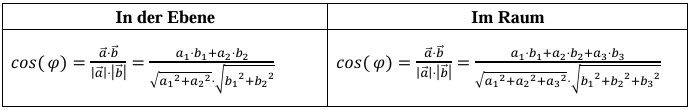
\includegraphics[width=\linewidth]{images/vec-winkel.png}
        \end{center}
    \end{formula}
    
    \begin{theorem}{Winkel und Skalarprodukt}

        
        \begin{wrapfigure}{r}{0.4\linewidth}
            \vspace{-20pt}
            \begin{align*}
                \phi<\frac{pi}{2},\, \text{ wenn } \vec{a}\cdot\vec{b} > 0 \text{ ist.}\\    
                \phi>\frac{pi}{2},\, \text{ wenn } \vec{a}\cdot\vec{b} < 0 \text{ ist.}\\    
                \phi=\frac{pi}{2},\, \text{ wenn } \vec{a}\cdot\vec{b} = 0 \text{ ist.}    
            \end{align*}
        \end{wrapfigure}
        Seien $\vec{a}$ und $\vec{b}$ zwei Vektoren und $\phi$ der eingeschlossene Winkel, 
        $0\leq\phi\leq\pi$, dann gilt:
        \vspace{40pt}
    \end{theorem}

    \begin{formula}{Orthogonal Projektion}\\
        Für die orthogonale Projektion $\vec{b}_a$ eines Vektors $\vec{b}$ auf einen Vektor $\vec{a}$ gilt:


        \vspace{-10pt}
        \begin{wrapfigure}{r}{0.3\linewidth}
            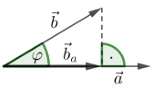
\includegraphics[width=0.9\linewidth]{images/vec-proj.png}
        \end{wrapfigure}
        \begin{align*}
            \vec{b}_a=\frac{\vec{a}\cdot\vec{b}}{\abs{\vec{a}}^2}\cdot\vec{a}   
            \text{ und }
            \abs{\vec{b}}_a=\frac{\abs{\vec{a}\cdot\vec{b}}}{\abs{\vec{a}}}   
        \end{align*}
        Die erste Formel gilt für den Fall $0\leq\phi\leq\frac{\pi}{2}$,
        die zweite für $\frac{\pi}{2}<\phi\leq\pi$
    \end{formula}

    \begin{definition}{Vektorprodukt}
        \begin{wrapfigure}{r}{0.3\linewidth}
            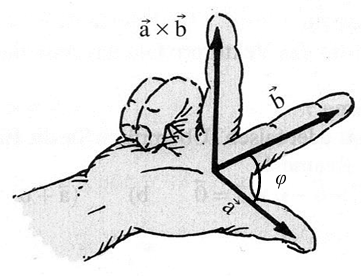
\includegraphics[width=0.9\linewidth]{images/vec-hand.png}
        \end{wrapfigure}
        Das \textit{Vektorprodukt} $\vec{a}\times\vec{b}$ zweier räumlicher Vektoren $\vec{a}$ und $\vec{b}$
        ist der eindeutig bestimmte Vektor mit folgenden Eigenschaften:¨
        \begin{itemize}
            \item $\vec{a}\times\vec{b}$ \textbf{ist orthogonal zu } $\vec{b}$ \textbf{ und zu } $\vec{b}$.
            \item $\abs{\vec{a}\times\vec{b}}=\abs{\vec{a}}\cdot\abs{\vec{b}}\cdot\sin(\phi)$
            \item $\vec{a}, \vec{b}$ und $\vec{a}\times\vec{b}$ bilden (in dieser Reihenfolge!) 
                ein \textit{Rechtssystem}: Wenn Der Daumen der rechten Hand in die Richtung von $\vec{a}$
                zeigt und der Zeigefinger in die Richtung von $\vec{b}$, dann gibt der Mittelfinger die
                Ausrichtung von $\vec{a}\times\vec{b}$ an.
        \end{itemize}
        Dabei ist $\phi$ der Zwischenwinkel zwischen $\vec{a}$ und $\vec{b} (0\leq\phi\leq\phi)$.
        Wir definieren aussderem: $\vec{a}\times\vec{0}=\vec{b}\times\vec{0}=\vec{0}$.
    \end{definition}

    \begin{theorem}{Eigenschaften des Vektorprodukt}\\
        Für beliebige Vektoren $\vec{a}, \vec{b}$ und $\vec{c}$ sowie für jede beliebiges $\lambda\in R$ gilt:
        \begin{itemize}
            \item $\vec{a}, \vec{b}$ \textbf{ sind genau dann kollinear, wenn } $\vec{a}\times\vec{b}=\vec{0}$
            \item $\vec{a}\times\vec{a}=\vec{0}$
            \item Antikommutativ-Gesetz: $\vec{a}\times\vec{b}=-(\vec{b}\times\vec{a})$
            \item Distributiv-Gesetz: $\vec{a}\times(\vec{b}+\vec{c})=\vec{a}\times\vec{b}+\vec{a}\times\vec{c}$
            \item Gemmischtes Assoziativ-Gesetz\\
                $\lambda\cdot(\vec{a}\times\vec{b})=(\lambda\cdot\vec{a})\times\vec{b}=\vec{a}\times(\lambda\cdot\vec{b})$ 
        \end{itemize}
        \begin{highlight}{<!>}
            Das normale Assoziativ-Gesetz gilt im Allgemeinen nicht ($\vec{a}\times(\vec{b}\times\vec{c})\ne(\vec{a}\times\vec{b})\times\vec{c}$)!
        \end{highlight}
    \end{theorem}

    \begin{formula}{Vektorproduktes aus der Komponentendarstellung}\\
        \begin{minipage}[c]{0.5\linewidth}
            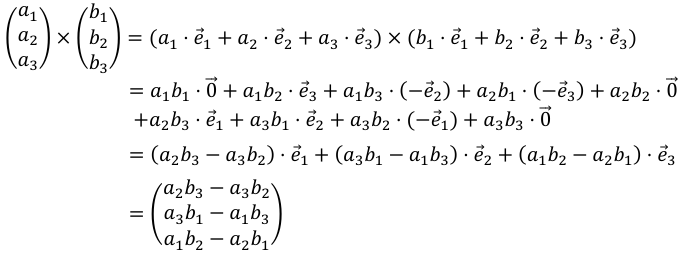
\includegraphics[width=0.8\linewidth]{images/vec-prod-form.png}
        \end{minipage}
        \begin{minipage}[c]{0.5\linewidth}
            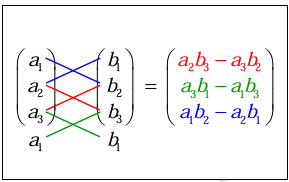
\includegraphics[width=0.8\linewidth]{images/vec-prod.png}
        \end{minipage}
    \end{formula}

    \begin{formula}{Vektorprodukt und Fläche des Parallelogramms}\\
        Der Betrag des Vektorproduktes $\vec{a}\times\vec{b}$ ist gleich dem Flächeninhalt des von 
        $\vec{a}$ und $\vec{b}$ aufgespannten Parallelogramms.
    \end{formula}

    \begin{theorem}{Lage von Geraden im Raum}
        \begin{center}
            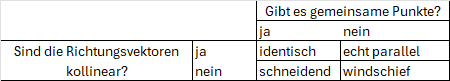
\includegraphics[width=0.8\linewidth]{images/geraden-lage-raum.png}
        \end{center}
    \end{theorem}

    \begin{definition}{Parameterdarstellung}
        \begin{wrapfigure}{r}{0.3\linewidth}
            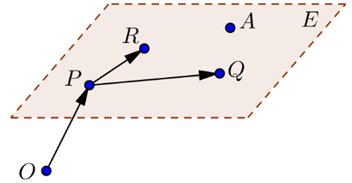
\includegraphics[width=0.9\linewidth]{images/vec-param.png}
        \end{wrapfigure}
        Eine Gerade oder Ebene $E$ lässt sich durch eine Gleichung der folgenden Form beschreiben:
        \begin{equation*}
            E:\,\vec{r}(P)+\lambda\cdot\vec{a}+\mu\cdot\vec{b}\, (\lambda,\mu\in\R)
        \end{equation*}
        Der Punkt $P$ heisst \textit{Aufpunkt}, die Vektoren $a=\overrightarrow{PQ}$ und 
        $\vec{b}=\overrightarrow{PR}$ heissen \textit{Richtungsvektoren} von $E$.
        Die Parameterdarstellung ist nicht eindeutig. Als Richtungsvektoren werden zwei beliebige
        Vektor gewählt, die \textit{parallel} zu $E$ sind und \textit{nicht kollinear} sind.
    \end{definition}

    \begin{definition}{Koordinatendarstellung}\\
        Eine Ebene $E$ im Raum lässt sich durch eine Gleichung der folgenden Form Beschreiben:
        \begin{equation*}
            E:\,ax+by+cz+d=0,\, \text{mit } a,b,c,d\in \R
        \end{equation*}
        Dait ist gemeint, dass die Ebene E aus allen Punkten $P$ besteht, deren Koordinaten
        $x, y$ und $z$ diese Gleichung erfüllen.
        Das $\abs{d}$ stellt den Abstand zum Ursprung dar, wenn die Gleichung normiert ist. 
        Ansonsten ist es $\frac{\vec{d}}{\vec{n}}$ 
    \end{definition}

    \begin{formula}{Umrechnung Parameterdarstellung zu Koordinatendarstellung}\\
        Für das Berechnen der Koordinatendarstellung aus der Parameterdarstellung gibt es mehrere
        Möglichkeiten.

        Die Einfachste ist das berechnen über den Normalenvektor aus dem Kreuzprodukt der Richtungsvektoren,
        welches die Koeffizienten $a, b$ und $c$ liefert.
        \begin{equation*}
            \vec{n}=\vec{a}\times\vec{b}=\begin{psmallmatrix}
                a\\b\\c
            \end{psmallmatrix}
        \end{equation*}
        Der Aufpunkt wird über das Einsetzen eines Punktes der Ebene $E$ ermittelt.

        Die zweite Möglichkeit ist es, ein LGS aufzustellen und die Parameter zu eliminieren.
        \begin{equation*}
            \vec{r}(P)+\lambda\cdot\vec{a}+\mu\cdot\vec{b}=\begin{psmallmatrix}
                x\\y\\z
            \end{psmallmatrix}
        \end{equation*}
    \end{formula}

    \begin{formula}{Umrechnung Koordinatendarstellung zu Parameterdarstellung}\\
        Um eine Koordinatendarstellung in eine Parameterdarstellung umzurechnen,
        werden drei Punkte berechnet.
        Einer dieser Punkte wird dann als aufpunkt gewählt und mit den restlichen
        werden Richtungsvektoren berechnet.
    \end{formula}

    \begin{formula}{Abstand Punkt-Gerade}\\
        Für das finden des Abstandes zu einer Geraden gibt es verschiedene Möglichkeit.\\
        \textbf{Hier der Weg über den Fusspunkt.}
        Gegeben Gerade $g=\vec{r}(P)+\lambda\cdot\vec{a}$ in Parameterform und Punkt $A$. Gesucht ist der Fusspunkt $B\in g$.
        \begin{wrapfigure}{r}{0.3\linewidth}
            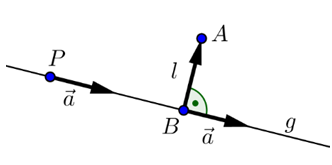
\includegraphics[width=0.8\linewidth]{images/vec-abstand-von-punkt.png}
        \end{wrapfigure}
        \begin{enumerate}
            \item Da $B\in g\Rightarrow \vec{r}(B)=\begin{psmallmatrix}
                P_x+a\lambda_B\\
                P_y+b\lambda_B\\
                P_z+c\lambda_B
            \end{psmallmatrix}$. 
            \item Da $\overrightarrow{BA}\perp g\Rightarrow\overrightarrow{BA}\cdot\vec{a}=0$
            \item Jetzt kann ein LGS aufgestellt und aufgelöst werden.
        \end{enumerate}
        Weiter Möglichkeit gehen über die Projektion oder die Fläche des Kreuzprodukt.
    \end{formula}

    \begin{formula}{Abstand Punkt-Ebene}


        \begin{wrapfigure}{r}{0.3\linewidth}
            \vspace{-10pt}
            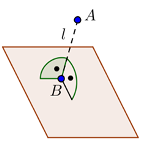
\includegraphics[width=0.7\linewidth]{images/vec-abstand-von-ebene.png}
            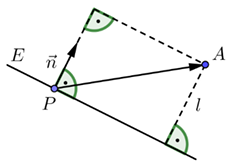
\includegraphics[width=0.7\linewidth]{images/vec-abstand-von-ebene2.png}
        \end{wrapfigure}
        Gegeben ein Punkt $A=(x_A;y_A;z_A)$ sowie eine Ebene $E$ mit der \textbf{normierten} 
        Koordinatendarstellung $E:\,ax+by+cz+d=0$.
        Dann gilt für den Abstand $l$ des Punktes $A$ von der Ebene $E$ die gleichung (1).
        Ist die Koordinatendarstellung nicht \textbf{nicht normiert}, so gilt (2).
        \begin{align}
            l=\abs{ax_A+by_A+cz_A+d}\\
            l=\frac{\abs{ax_A+by_A+cz_A+d}}{\abs{\vec{n}}}
        \end{align}
    \end{formula}